\section{O que já foi feito}

\subsection{Lista de requisitos funcionais e não funcionais}
\subsubsection{Lista de requisitos funcionais}

\renewcommand{\arraystretch}{1.3}
\begin{center} % Centralizar a tabela
\begin{longtable}{|c|p{9cm}|c|} % Reduzi a largura da coluna de descrição
    \hline
    \textbf{Referência} & \textbf{Descrição} & \textbf{Prioridade} \\
    \hline
    RF01 & Eu, como utilizador, quero criar uma conta para poder aceder à plataforma e usufruir dos serviços. & Alta \\
    \hline
    RF02 & Eu, como utilizador, quero fazer \textit{login} para poder aceder à minha conta e \textit{gerenciar} os meus dados. & Alta \\
    \hline
    RF03 & Eu, como utilizador, quero criar e editar \textit{skills} para poder associá-las a talentos e melhorar a minha pesquisa e gestão de profissionais. & Alta \\
    \hline
    RF04 & Eu, como utilizador, quero apagar uma \textit{skill} apenas se ela não estiver associada a nenhum talento para garantir a consistência dos dados. & Alta \\
    \hline
    RF05 & Eu, como utilizador, quero pesquisar talentos por uma combinação de \textit{skills} para encontrar o profissional adequado para as necessidades de um cliente ou projeto. & Alta \\
    \hline
    RF06 & Eu, como utilizador, quero gerar um relatório com o preço médio mensal por categoria de talento e por país para analisar as tendências salariais e tomar decisões informadas. & Alta \\
    \hline
    RF07 & Eu, como utilizador, quero gerar um relatório com o preço médio mensal por \textit{skill} para avaliar as competências mais valorizadas no mercado e ajustar as estratégias de contratação. & Alta \\
    \hline
    RF08 & Eu, como cliente, quero criar um cliente na plataforma para associar talentos às minhas necessidades de contratação. & Alta \\
    \hline
    RF09 & Eu, como cliente, quero criar uma proposta de trabalho para definir o tipo de talento que procuro e as \textit{skills} necessárias para esse trabalho. & Alta \\
    \hline
    RF10 & Eu, como cliente, quero associar \textit{skills} a uma proposta de trabalho para especificar as competências necessárias para o trabalho. & Alta \\
    \hline
    RF11 & Eu, como cliente, quero registrar o número de anos de experiência mínima por \textit{skill} para garantir que os talentos atendem aos requisitos do trabalho. & Alta \\
    \hline
    RF12 & Eu, como cliente, quero indicar o número total de horas e a descrição do trabalho para que os talentos saibam o que é esperado. & Alta \\
    \hline
    RF13 & Eu, como cliente, quero atualizar ou remover uma proposta de trabalho para manter as oportunidades de emprego atualizadas. & Alta \\
    \hline
    RF14 & Eu, como cliente, quero listar todos os talentos elegíveis para uma proposta de trabalho, ordenados pelo valor total, para facilitar a escolha do profissional mais adequado. & Alta \\
    \hline
    RF15 & Eu, como talento, quero criar um perfil com informações como nome, país, e-mail e preço por hora para me apresentar de forma profissional na plataforma. & Alta \\
    \hline
    RF16 & Eu, como talento, quero definir a visibilidade do meu perfil como público ou privado para controlar quem pode ver as minhas informações. & Alta \\
    \hline
    RF17 & Eu, como talento, quero associar várias \textit{skills} ao meu perfil, indicando os anos de experiência em cada \textit{skill}, para destacar as minhas competências. & Alta \\
    \hline
    RF18 & Eu, como talento, quero adicionar experiências profissionais ao meu perfil, incluindo o título, nome da empresa e anos de experiência, para demonstrar o meu histórico profissional. & Alta \\
    \hline
    RF19 & Eu, como talento, quero garantir que não haja sobreposição de períodos de experiência no meu perfil para manter a consistência dos dados. & Baixa \\
    \hline
\end{longtable}
\end{center}

\subsubsection{Requisitos Não Funcionais}

\renewcommand{\arraystretch}{1.3}
\begin{center} % Centralizar a tabela
\begin{longtable}{|c|p{11.35cm}|} % Reduzi a largura da coluna de descrição
    \hline
    \textbf{Referência} & \textbf{Descrição} \\
    \hline
    RNF01 & O Software será desenvolvido na linguagem C\# \\
    \hline
    RNF02 & O Software estabelecerá ligação com a base de dados PostgreSQL \\
    \hline
\end{longtable}
\end{center}

\newpage

\subsection{Modelo de caso de uso}
\begin{figure}[h]
    \centering
    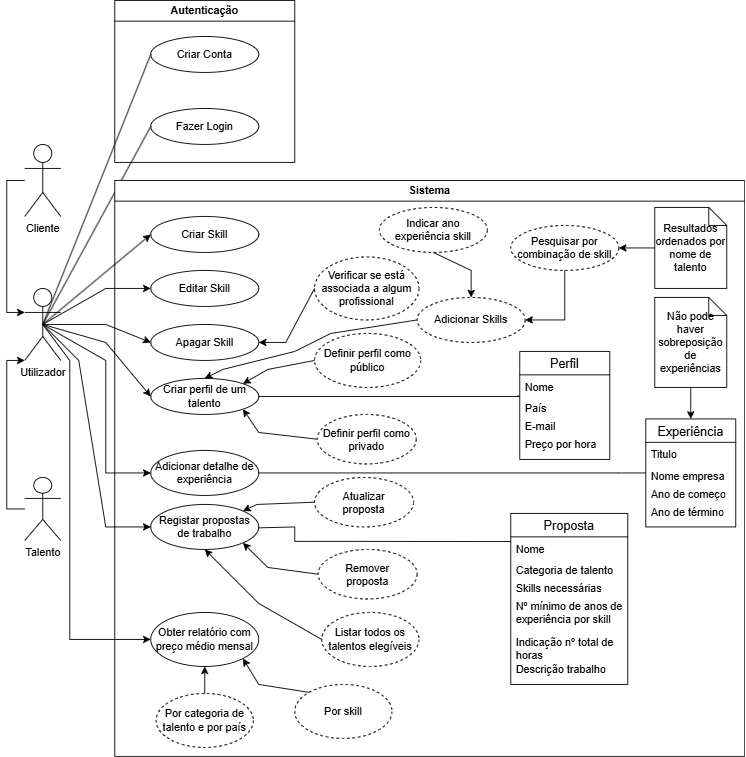
\includegraphics[width=1\linewidth]{imagens/casosdeuso.drawio.png}
    \caption{Modelo de casos de uso}
    \label{fig:1}
\end{figure}

\newpage

\subsection{Modelo de classes}

\begin{figure}[h]
    \centering
    
\includegraphics[width=1\linewidth]{imagens/ModeloDominio_v2.png}
    \caption{Modelo de domínio}
    \label{fig:2}
\end{figure}

\newpage

\subsection{Lista de tarefas}

\renewcommand{\arraystretch}{1.3}
\begin{center} % Centralizar a tabela
\begin{longtable}{|c|p{7cm}|c|}
\hline
\textbf{Pessoa} & \textbf{Descrição} & \textbf{Nível de esforço} \\
\hline
Daniel Gonçalves & Criar Lista de Requisitos & 2 \\
\hline
João Rodrigues & Criar diagrama de domínios & 2 \\
\hline
João Rodrigues & Criar diagrama de casos de uso & 2 \\
\hline
Gonçalo Carneiro & Criar lista de tarefas & 2 \\
\hline
Micael costa & Criar Modelo de Base de Dados & 2 \\
\hline
 & Criação da Base de Dados & 3 \\
\hline
 & Implementar a funcionalidade de criação de conta e login de utilizadores & 5 \\
\hline
 & Implementar o módulo de criação e edição de skills & 5 \\
\hline
 & Desenvolver a funcionalidade de criação e gestão de perfis de talentos & 5 \\
\hline
 & Implementar a funcionalidade para pesquisa de talentos através de uma combinação de skills, ordenado por nome & 3 \\
\hline
 & Criar o sistema de propostas de trabalho, permitindo edição e remoção & 8 \\
\hline
 & Desenvolver a funcionalidade de pesquisa de talentos com ordenação por nome & 3 \\
\hline
 & Desenvolver o registo de propostas de trabalho por parte de um utilizador & 5 \\
\hline
 & Implementar a listagem de talentos elegíveis para propostas, ordenados por valor total & 3 \\
\hline
 & Criar relatórios de preço médio mensal por categoria de talento e por país & 3 \\
\hline
 & Criar relatórios de preço médio mensal por skill & 3 \\
\hline
 & Implementação da introdução de várias skills para um perfil de talento & 5 \\
\hline
 & Desenvolver a possibilidade de adição de uma determinada experiência & 8 \\
\hline
\end{longtable}
\end{center}


\subsection{Base de dados}
\subsubsection{Diagrama DER da base de dados}
\begin{figure}[h]
    \centering
    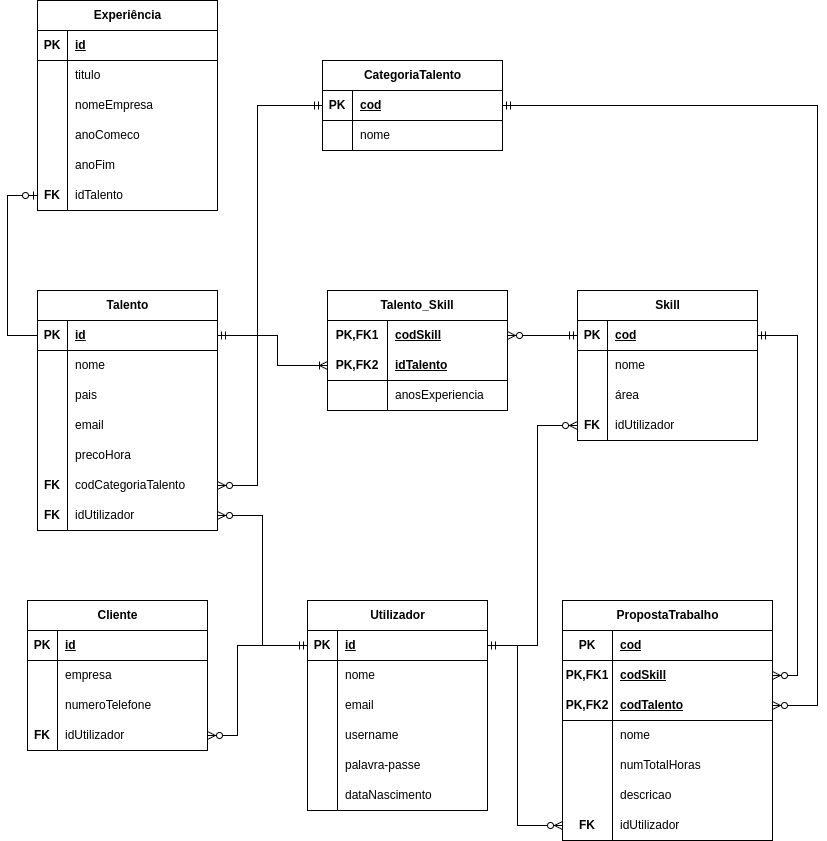
\includegraphics[width=1\linewidth]{imagens/derbd.png}
    \caption{Diagrama da base de dados}
    \label{fig:}
\end{figure}

\subsubsection{Script para criação da base de dados}
\begin{lstlisting}[language=SQL]
-- Table: Utilizador
CREATE TABLE Utilizador (
    id SERIAL PRIMARY KEY,
    nome VARCHAR(255) NOT NULL,
    email VARCHAR(255) UNIQUE NOT NULL,
    username VARCHAR(50) UNIQUE NOT NULL,
    "palavra-passe" VARCHAR(255) NOT NULL,
    dataNascimento DATE NOT NULL
);

-- Table: Cliente
CREATE TABLE Cliente (
    id SERIAL PRIMARY KEY,
    empresa VARCHAR(255) NOT NULL,
    numeroTelefone VARCHAR(20) NOT NULL,
    idUtilizador INT NOT NULL REFERENCES Utilizador(id)
);

-- Table: CategoriaTalento
CREATE TABLE CategoriaTalento (
    cod SERIAL PRIMARY KEY,
    nome VARCHAR(255) NOT NULL
);

-- Table: Talento
CREATE TABLE Talento (
    id SERIAL PRIMARY KEY,
    nome VARCHAR(255) NOT NULL,
    pais VARCHAR(100) NOT NULL,
    email VARCHAR(255) UNIQUE NOT NULL,
    precoHora DECIMAL(10, 2) NOT NULL,
    codCategoriaTalento INT REFERENCES CategoriaTalento(cod),
    idUtilizador INT NOT NULL REFERENCES Utilizador(id)
);

-- Table: Experiência
CREATE TABLE Experiencia (
    id SERIAL PRIMARY KEY,
    titulo VARCHAR(255) NOT NULL,
    nomeEmpresa VARCHAR(255) NOT NULL,
    anoComeco INT NOT NULL,
    anoFim INT,
    idTalento INT NOT NULL REFERENCES Talento(id)
);

-- Table: Skill
CREATE TABLE Skill (
    cod SERIAL PRIMARY KEY,
    nome VARCHAR(255) NOT NULL,
    area VARCHAR(255),
    idUtilizador INT REFERENCES Utilizador(id)
);

-- Table: Talento_Skill (junction table for Talento and Skill)
CREATE TABLE Talento_Skill (
    codSkill INT NOT NULL REFERENCES Skill(cod),
    idTalento INT NOT NULL REFERENCES Talento(id),
    anosExperiencia INT NOT NULL,
    PRIMARY KEY (codSkill, idTalento)
);

-- Table: PropostaTrabalho
CREATE TABLE PropostaTrabalho (
    cod SERIAL PRIMARY KEY,
    codSkill INT NOT NULL REFERENCES Skill(cod),
    codTalento INT NOT NULL REFERENCES Talento(id),
    nome VARCHAR(255) NOT NULL,
    numTotalHoras INT NOT NULL,
    descricao TEXT,
    idUtilizador INT REFERENCES Utilizador(id),
    UNIQUE (codSkill, codTalento)
);
\end{lstlisting}